\documentclass[letterpaper,12pt,oneside]{book}
\usepackage[utf8]{inputenc}
% To ensure every single paragraph is indented.
\usepackage{indentfirst}
% For image importing
\usepackage{graphicx}
% hyperref is to ensure chapters and other anchors
% are a clickable link.
\usepackage[pdfpagelabels=false]{hyperref}
% For better floating of images
\usepackage{stfloats}


\title{Natron For Newbies\\Version: Early Working Draft.}
\author{Written By: Matthew Polk}
\date{}

\begin{document}
% I want everything up till the first actual page to be blank.
\addtocontents{toc}{\protect\thispagestyle{empty}}
%%<----------------------------------------------------------------------------------------->
% Bit of trickery to get the title page and TOC the way I wanted it.
% I renamed the default contents name to be more clear for the
% end user reading it.
\renewcommand{\contentsname}{Table of Contents}
% I had to do a few workaround to ensure the title page was blank
% for page numbering and the TOC was using roman numerals
% instead of regular 1,2,3,4....
\frontmatter
\hypersetup{pageanchor=false}
\maketitle
\hypersetup{pageanchor=true}

\tableofcontents
\cleardoublepage


\mainmatter

% Main matter is when the main contents of the document begins.
%%<--------------------------------------------------------------------------------->

\part{Using Natron}
% Part one will be dedicated to how to use natron without how to
% extending it using python or GLSL or anything like that.

\chapter{What Is Natron?}
Welcome aboard, natron is very powerful but takes a bit of learning to
fully utilize. This chapter is about introducing you to the program.

\bigbreak
\section{Introduction}
Natron is a GPL-2.0 licensed visual effect compositor that is very similar to nuke. If you've used nuke, you'll get the hang of natron very quickly. But this document is not just for those wanting to get up to speed with natron if already familiar with nuke. It's also for those who are used to after effects or even have never done compositing before. It really is just a few fundamentals to understand, because they flow between other programs considerably.
\newpage

\begin{figure}[!t]
\vspace*{-1in}
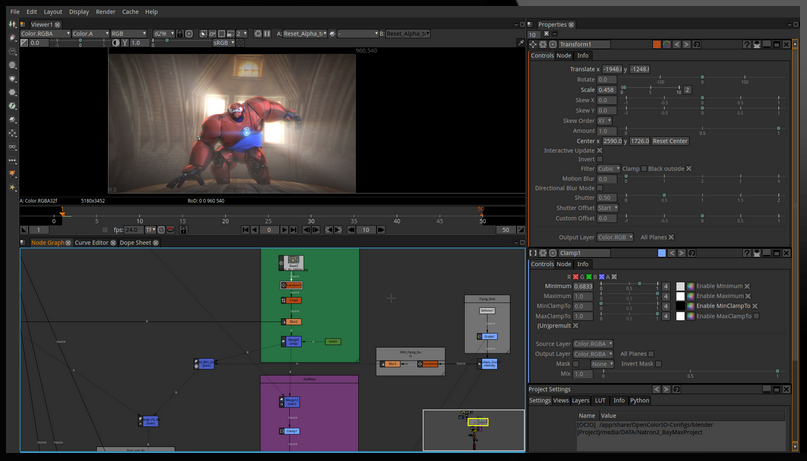
\includegraphics[width=\linewidth,height=6in]{./imgs/Natron.png}
\caption{Natron GUI In Action}
\end{figure}



\newpage
As pictured above, you'll see several aspects of the natron user interface. FIrstly, to the left, are shortcuts for node groups. To the upper right of that, is the preview area of your clips you're working with. Below that, is the working area for nodes and to the right are properties for every node placed in the working area.

\newpage

\section{Nodes}
\noindent
What is a node?
\bigbreak
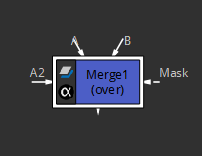
\includegraphics{./imgs/mergenode.png}
\bigbreak
A node like pictured above, can be described as like a lego brick.
You connect input and output ports to modify the results as you desire.
To me, nodes are far more powerful and flexible compared to layer based compositing such as after effects.

Don't be intimidated by how often you see complex webs for node trees, only use what nodes you truly need. Less is more, Keep It Simple Stupid (KISS Principle) should be rule of thumb here.

\section{File Formats To Use}

\chapter{Compositing Fundamentals}

\section{Mattees}
Luma-Key, Chroma-Key, Difference, Color-Difference, etc.

\section{Despill}

\section{Composite}

\section{Blending}

\section{Gamma}

\section{RGBA}

\section{Log}

\section{Linear}

\section{Masks}

\section{Green Screen}

\section{Blue Screen}

\section{Motion Tracking}

\section{YUV HSV Floating Point}

\section{3D}

\chapter{Examples Of Using Natron}




%%End Of Part 1
%%<------------------------------------------------------------------------------------->
\part{Extending Natron}
% Part two will be to how to use languages such as python or GLSL
% to extend natron further should you desire to.

\chapter{Python API}




\chapter{GLSL}



\chapter{GMic}




\end{document}
